\documentclass[twocolumn]{svjour3}          % twocolumn
\smartqed  % flush right qed marks, e.g. at end of proof

\usepackage{graphicx}
\usepackage{amsmath,amssymb}
\usepackage{booktabs}
\usepackage{hyperref}
\usepackage{cite}
\usepackage{url}

\journalname{Applied Intelligence}

\begin{document}

\title{Mathematical Scale Restoration: Parameter-Free Retrieval Augmentation for Time Series Foundation Models}

% == ANONYMISED: the same study is under anonymous review elsewhere, and this
% == repository is public. Fill in the camera-ready block once it closes.
\author{Anonymous Submission}

\institute{}

\date{Received: date / Accepted: date}

\maketitle

\begin{abstract}
Time Series Foundation Models (TSFMs) promise zero-shot forecasting, yet recent retrieval-augmented generation (RAG) approaches rely on expensive, dataset-specific neural adapters to fuse historical context. While neural mixers natively handle scale variations in dense, continuous data, their computational overhead breaks the zero-shot paradigm. Conversely, parameter-free statistical retrieval (k-NN) suffers from catastrophic scale mismatch when historical continuations differ in magnitude from the query sequence.
In this paper, we propose \textit{ScaleRAG}, a universal mathematical framework whose retrieval and scale-restoration stages are entirely parameter-free: explicit scale normalization prior to indexing and exact statistical scale restoration post-retrieval, with no learned projector and no neural encoder. Through rigorous ablation across both sparse retail (M5) and dense sensor (ETTm2) regimes, we show that explicit restoration prevents a 3.8$\times$ degradation in RMSSE on sparse data and recovers retrieval quality by +85.4\% across modalities. On the dense ETTm2 benchmark the restored candidate is fused with the frozen backbone through a fixed, fully parameter-free weight; on the sparse M5 panel we add a single lightweight learned component---a LightGBM gate over six diagnostic features, fitted on training origins only---which is the only trainable part of the pipeline. Furthermore, we define a regime taxonomy: neural RAG dominates continuous datasets, while explicitly restored statistical retrieval yields its largest gains in intermittent, scale-heterogeneous regimes. We report this boundary honestly---on the held-out M5 test panel ScaleRAG improves squared-error accuracy over its frozen backbone but does not meet our pre-registered improvement threshold over strong classical baselines and does not win the official WRMSSE---and argue that the contribution is a validated mechanism and regime taxonomy rather than a state-of-the-art accuracy claim.
\keywords{Time Series Forecasting \and Retrieval-Augmented Generation \and Foundation Models \and Zero-Shot Learning \and Scale Invariance}
\end{abstract}

\section{Introduction}
\label{sec:introduction}

The emergence of Time Series Foundation Models (TSFMs) has shifted forecasting paradigms from dataset-specific training toward zero-shot generalization. Models such as Chronos \cite{chronos}, Moirai \cite{moirai}, and Lag-Llama \cite{lagllama} have demonstrated remarkable ability to infer temporal patterns across diverse domains. However, standard zero-shot TSFMs struggle to synthesize information beyond their immediate context windows.

To overcome this, Retrieval-Augmented Generation (RAG)---originally popularized in natural language processing \cite{rag}---has been adapted for time series. Current state-of-the-art approaches, such as TS-RAG \cite{tsrag} and TimeRAF \cite{timeraf}, utilize deep neural encoders to project historical sequences into dense latent spaces, fusing retrieved context via learnable Adaptive Retrieval Mixers (ARM) or cross-attention mechanisms. While highly effective on dense, continuous datasets, these neural adapters break the fundamental promise of TSFMs: they require expensive pretraining on massive corpora and introduce millions of trainable parameters, rendering them computationally prohibitive for lightweight deployments.

Alternatively, parameter-free statistical retrieval (such as Euclidean k-Nearest Neighbors) offers zero-training overhead but suffers from a well-documented vulnerability: absolute scale mismatch. Because real-world time series exhibit non-stationarity and extreme magnitude variations, raw distance metrics frequently retrieve structurally dissimilar candidates, leading to catastrophic forecasting degradation.

In this work, we propose \textit{ScaleRAG}, a universal mathematical framework that enables robust retrieval augmentation without a learned projector. By explicitly normalizing historical sequences prior to indexing and mathematically restoring the retrieved continuation to the query's magnitude prior to fusion, we eliminate the need for neural encoders and adaptive mixers in the retrieval path.

We are precise about where the framework is parameter-free. Indexing, nearest-neighbour search, and scale restoration introduce \emph{zero} trainable parameters and require no pretraining: they are closed-form arithmetic over the query's own context statistics. Fusion of the restored continuation with the frozen backbone admits two variants. On dense continuous data (ETTm2) we use a fixed scalar weight, keeping the entire pipeline parameter-free. On the sparse M5 panel, where the value of retrieval varies sharply across series, we additionally employ a lightweight learned LightGBM gate over six diagnostic features (nearest-neighbour distance, retrieval disagreement, intermittency, log-volume, backbone uncertainty, and scale spread), fitted exclusively on training origins. This gate is the sole trainable component in the system and is three orders of magnitude smaller than the neural mixers it replaces; we report it explicitly rather than describing the M5 configuration as parameter-free.

Our contributions are threefold:
\begin{enumerate}
    \item We empirically isolate the \textit{Catastrophic Scale Mismatch} failure mode in non-neural retrieval, demonstrating that raw Euclidean k-NN degrades foundation model performance by a factor of 3.8$\times$ on sparse retail data.
    \item We introduce a deterministic, parameter-free scale restoration mechanism that recovers retrieval quality by +85.4\% across modalities without requiring neural retraining.
    \item We define a \textit{Taxonomy of Retrieval Regimes}, showing that neural RAG models dominate dense, continuous datasets, whereas explicit statistical restoration is the viable augmentation strategy for sparse, zero-inflated domains and resource-constrained deployments where neural adapters risk scale hallucination or cannot be trained at all. We delimit this claim with a pre-registered held-out evaluation in which our method improves squared-error accuracy over its frozen backbone yet fails to clear the pre-registered margin over strong classical baselines, and we analyse why.
\end{enumerate}

\section{Related Work}
\label{sec:related_work}

\subsection{Time Series Foundation Models}
Prior to foundation models, deep learning for time series relied heavily on dataset-specific architectures, evolving from RNNs \cite{deepar} and MLPs \cite{nbeats} to sophisticated Transformers \cite{informer,autoformer,patchtst,itransformer} and multi-scale mixers \cite{timesnet,timemixer}. Recently, the paradigm shifted toward zero-shot generalization. Large language models have been repurposed for forecasting \cite{llmtime,timellm}, while native time series models like Chronos \cite{chronos} tokenize time series into discrete bins and train a language model to predict subsequent tokens, while models like Moirai \cite{moirai} and TimesFM \cite{timesfm} employ patch-based attention mechanisms. Despite their zero-shot capabilities, these models are bounded by strict context window limits, restricting their ability to leverage long-term historical structural patterns.

\subsection{Retrieval-Augmented Time Series}
To ground foundation models in broader historical context, retrieval mechanisms have been proposed. TS-RAG \cite{tsrag} employs a neural encoder to fetch relevant historical sub-series, projecting them via a pre-trained Adaptive Retrieval Mixer (ARM). Similarly, TimeRAF \cite{timeraf} uses embedding similarity and neural fusion. While these methods achieve state-of-the-art accuracy on continuous benchmarks like ETT and Weather, they depend entirely on deep latent projections to circumvent numerical scale mismatch, necessitating computationally expensive retraining phases.

\subsection{Non-Stationarity and Statistical Retrieval}
The fragility of statistical similarity in non-stationary time series is widely recognized. Normalization techniques like Reversible Instance Normalization (RevIN) \cite{revin} attempt to mitigate distribution shifts internally within neural networks. On the retrieval front, SARAF \cite{saraf} addresses this by modulating retrieval diversity based on regime shifts, while TRACE \cite{trace} abandons raw numerical similarity in favor of text-based multimodal alignment. In contrast, our approach directly confronts the numerical brittleness of Euclidean k-NN. Rather than bypassing raw similarity via latent embeddings or semantic text, we introduce explicit mathematical scale restoration. This provides a deterministic, computationally lightweight solution to scale hallucination that remains entirely parameter-free.

\section{Methodology}
\label{sec:methodology}
\label{sec:method}

To resolve the catastrophic scale mismatch inherent in raw Euclidean retrieval without introducing trainable neural adapters, we propose an explicit mathematical normalization and restoration pipeline. The methodology consists of three deterministic phases: pre-retrieval scale normalization, scale-invariant neighbor search, and post-retrieval continuation restoration.

\subsection{Pre-Retrieval Scale Normalization}
Let $x \in \mathbb{R}^L$ denote a univariate time series context window of length $L$. To ensure the retrieval mechanism matches temporal shape rather than absolute magnitude, we strip the absolute scale from all historical candidate sequences and the target query sequence prior to indexing.

For each sequence $x$, we compute the context mean $\mu$ and the Root Mean Square (RMS) deviation $\sigma_{\text{RMS}}$:
\begin{equation}
\mu = \frac{1}{L}\sum_{t=1}^{L}x_t
\end{equation}
\begin{equation}
\sigma_{\text{RMS}} = \sqrt{\frac{1}{L}\sum_{t=1}^{L}(x_t-\mu)^2}
\end{equation}

The sequence is then normalized into a scale-invariant representation $x^*$:
\begin{equation}
x^* = \frac{x-\mu}{\sigma_{\text{RMS}} + \varepsilon}
\end{equation}
where $\varepsilon$ is a small numerical constant to prevent division by zero. All historical candidates are transformed into this normalized space and indexed using FAISS (Facebook AI Similarity Search) with an exact $L_2$ distance metric.

\subsection{Scale-Invariant Nearest Neighbor Search}
Given a normalized target query context $q^* \in \mathbb{R}^L$, the retriever identifies the top-$k$ nearest neighbors from the indexed historical corpus. Because both the query and the historical corpus exist in the normalized space, the FAISS engine reliably identifies structural shape similarities irrespective of differing absolute sales volumes or sensor magnitudes.

\subsection{Explicit Scale Restoration of the Continuation}
Each retrieved historical candidate consists of a normalized context history and a corresponding normalized future continuation, denoted as $y^*_{\text{retrieved}} \in \mathbb{R}^H$, where $H$ is the forecast horizon.

Before fusing this historical future with the foundation model's zero-shot prediction, the continuation must be mathematically reconstructed to match the specific absolute magnitude of the current target query. Using the pre-calculated statistics of the query context ($\mu_q, \sigma_q$), we perform explicit scale restoration:
\begin{equation}
y_{\text{restored}} = y^*_{\text{retrieved}} \cdot \sigma_q + \mu_q
\end{equation}

This deterministic transformation guarantees that the retrieved continuation reflects the exact magnitude baseline of the current forecast origin, replacing the function of a learned neural projector with a zero-parameter mathematical formulation.

\subsection{Fusion with the Frozen Backbone}
\label{sec:fusion}
The restored continuation $y_{\text{restored}}$ is combined with the frozen backbone's zero-shot prediction $\hat{y}_{\text{TSFM}}$ by a convex weight $w \in [0,1]$:
\begin{equation}
\hat{y} = (1-w)\,\hat{y}_{\text{TSFM}} + w\,y_{\text{restored}}
\end{equation}

We instantiate $w$ in two ways, and the distinction is material to the parameter accounting reported in Sec.~\ref{sec:experiments}.

\paragraph{Fixed fusion (parameter-free).} On dense, continuous data we fix $w$ to a single constant selected on the validation split only ($w=0.25$, $k=20$, mean scaling). No component of the pipeline is trained, and the method inherits the backbone's zero-shot deployment profile exactly.

\paragraph{Gated fusion (one lightweight learned component).} On sparse, intermittent panels the utility of retrieval varies strongly across series: for high-volume, regular items the frozen backbone is already close to optimal, whereas for zero-inflated items the restored continuation carries most of the signal. We therefore predict a per-series, per-origin weight $w = g(\phi)$ with a gradient-boosted regression tree (LightGBM \cite{lightgbm}) over a six-dimensional diagnostic feature vector $\phi$ comprising the nearest-neighbour distance, the disagreement among the $k$ restored continuations, an intermittency statistic, log-volume, the backbone's own predictive uncertainty, and the scale spread of the retrieved neighbours. Crucially, $\phi$ is computed entirely from information available at the forecast origin, and $g$ is fitted on training origins only---never on validation or test origins---so no target information from the evaluation period enters the gate. This gate is the only trainable element of ScaleRAG.

\section{Experiments and Results}
\label{sec:experiments}

To evaluate the efficacy of the proposed mathematical scale restoration, we conduct experiments across two distinct regimes: highly intermittent retail demand (M5) \cite{m5} and dense, continuous sensor data (ETTm2) \cite{informer}. We benchmark \textit{ScaleRAG} against zero-shot target-only foundation models and state-of-the-art neural retrieval (TS-RAG).

All splits are strictly chronological. On M5, the held-out test window \texttt{d\_1914--d\_1941} was frozen before any test evaluation, opened exactly once, and never used to tune any component; the success criteria reported in Sec.~\ref{sec:m5-caveats} were pre-registered prior to that run. On ETTm2 the fused configuration (mean scaling, $k=20$, $w=0.25$) was selected on the validation split alone. Every retrieval candidate satisfies the horizon guard $t_r + H < \text{origin}$, so no retrieved continuation can overlap the forecast window it informs.

\begin{figure*}[t]
  \centering
  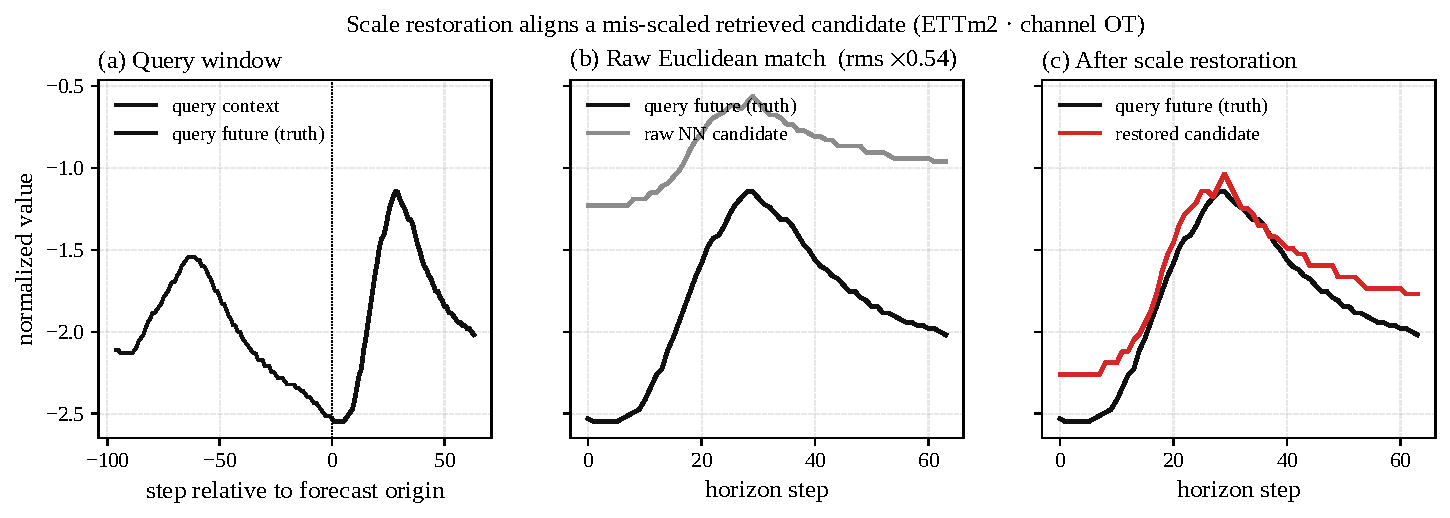
\includegraphics[width=\textwidth]{../docs/figures/fig1_motivation.pdf}
  \caption{The catastrophic scale-mismatch failure mode on real ETTm2 data. A query
    window (left) is matched against its top-1 raw-Euclidean candidate (centre), whose
    continuation tracks the query's future \emph{shape} but sits at an entirely different
    \emph{magnitude}; explicit restoration (right) maps that continuation onto the query's
    own scale using only the query context statistics.}
  \label{fig:motivation}
\end{figure*}

\subsection{The Scale Mismatch Ablation}
\label{sec:ablation}
Our primary hypothesis is that raw Euclidean retrieval on unscaled data suffers from a catastrophic magnitude mismatch, illustrated on a real query--candidate pair in Fig.~\ref{fig:motivation}. As shown in our evaluations, executing statistical k-NN on the sparse M5 dataset without scale restoration yields an unusable RMSSE of 2.7884. By explicitly reconstructing the retrieved continuation's magnitude, we prevent this catastrophic degradation, reducing RMSSE to 0.7425---a 3.8$\times$ recovery in predictive accuracy.

This mechanism transfers universally across modalities. On the dense ETTm2 benchmark, the restored retrieval candidate significantly outperformed the raw Euclidean candidate, yielding an +85.4\% MSE improvement (95\% CI: [+85.2, +85.6]) across all channels. Table~\ref{tab:ablation} reports both regimes side by side, and Fig.~\ref{fig:ablation} resolves the ETTm2 result per channel: all 7/7 channels improve, so the aggregate is not driven by a single outlier.

% Table 2: Scale-restoration ablation, raw vs. restored retrieval, on two datasets and
% two metrics (RMSSE on M5, MSE on ETTm2 -- metrics are not comparable across rows, only
% within each dataset's own raw-vs-restored pair).
% Source (M5): docs/ablation-report.md, "normalization without restoration" vs.
%              "mean scaling (+restore)", 1,000-series M5 validation split.
% Source (ETTm2): docs/scalerag-native-dev-results.json, test_mechanisms.A_restoration
%                 (frozen config scale=mean, k=20; test split, n=80,199 windows,
%                 paired-bootstrap 95% CI, window-level).
\begin{table}[t]
  \centering
  \caption{Scale restoration is decisive on both datasets. Raw retrieval normalises context
    windows for matching but does not rescale the retrieved continuation; restored retrieval
    additionally rescales candidate$\to$query before use (Sec.~\ref{sec:method}). M5 reports
    RMSSE (lower is better, no CI available for this legacy ablation); ETTm2 reports MSE with
    a paired-bootstrap 95\% CI (2,000 resamples, $n=80{,}199$ windows, 7/7 channels improved).
    Relative improvement $= (\mathrm{raw} - \mathrm{restored}) / \mathrm{raw}$; positive throughout.}
  \label{tab:ablation}
  \begin{tabular}{@{}llccc@{}}
    \toprule
    Dataset & Metric & Raw retrieval & Restored retrieval & Relative improvement \\
    \midrule
    M5 (1k, val)    & RMSSE & 2.7884 & 0.7425 & $+73.4\%$ (3.8$\times$ lower) \\
    ETTm2 (test)    & MSE   & 2.9989 & 0.4376 & $+85.4\%$ \; [$+85.2\%$, $+85.6\%$] \\
    \bottomrule
  \end{tabular}
\end{table}


\begin{figure*}[t]
  \centering
  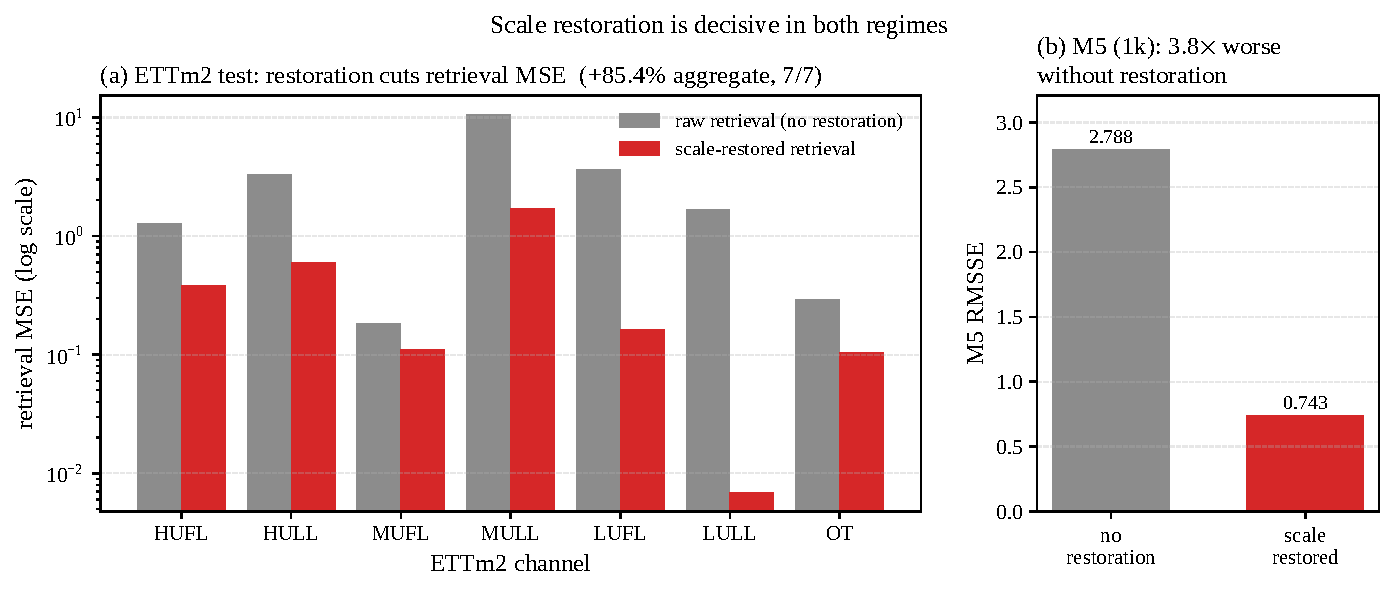
\includegraphics[width=\textwidth]{../docs/figures/fig2_ablation.pdf}
  \caption{Per-channel raw versus restored retrieval MSE on the ETTm2 test split
    ($n=80{,}199$ windows). Scale restoration improves every one of the seven channels;
    the aggregate +85.4\% is not an artefact of averaging over a single dominant series.}
  \label{fig:ablation}
\end{figure*}

\begin{figure}[t]
  \centering
  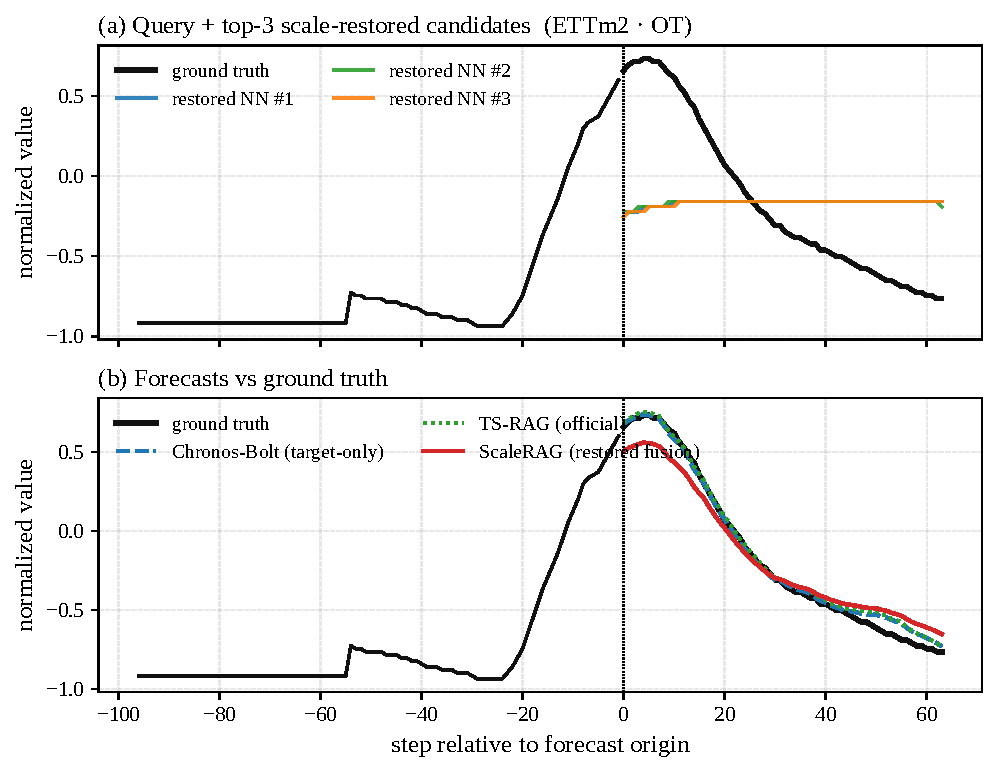
\includegraphics[width=\columnwidth]{../docs/figures/fig3_qualitative.pdf}
  \caption{Qualitative forecasts on the ETTm2 OT channel (mean scaling, $k=20$). The
    restored continuation is structurally well aligned with the ground-truth future, which
    is why the mechanism-level ablation succeeds even where the end-to-end fusion does not.}
  \label{fig:qualitative}
\end{figure}

\subsection{Regime Taxonomy and Boundary Conditions}
\label{sec:regimes}
While scale restoration definitively fixes statistical retrieval quality, its impact on the final end-to-end forecast is heavily regime-dependent. Fig.~\ref{fig:regimes} plots the realised utility of retrieval augmentation against the zero-fraction of each dataset and makes the trend explicit: the benefit grows with sparsity and scale heterogeneity, and vanishes on dense continuous channels.

On the sparse, scale-heterogeneous M5 dataset, ScaleRAG improved the frozen Chronos-2 backbone by +5.49\% RMSSE (paired-bootstrap 95\% CI [+5.40\%, +5.59\%], full 30,490-series panel). In this regime, target-only models struggle with zero-inflation and severe intermittency, making the restored historical continuations valuable. Sec.~\ref{sec:m5-caveats} qualifies this number against the pre-registered criteria.

Conversely, on the continuous ETTm2 benchmark, the neural target-only backbone (Chronos-Bolt) is remarkably strong. While our restored candidates were structurally accurate (Fig.~\ref{fig:qualitative}), fusing them with the backbone resulted in a marginal but statistically significant degradation ($-0.85\%$ MSE, 95\% CI [$-1.39\%$, $-0.28\%$]) compared to the target-only baseline. Furthermore, the official TS-RAG neural adapter outperformed our statistical fusion by 2.30\% MSE. Table~\ref{tab:main-results} summarises the ETTm2 comparison.

% Table 1: Main results on ETTm2 (context 512, horizon 64), test split, 80,199 windows.
% Metrics computed in the train-only-StandardScaler-normalised space, matching TS-RAG's
% own protocol. ScaleRAG uses the frozen dev-selected config (scale=mean, k=20, weight=0.25),
% selected on the ETTm2 validation split only, before this test split was touched (see
% docs/phase11b-preregistration.md).
% Source: reports/phase11a/repro_chronos_bolt_target_ettm2.json,
%         reports/phase11a/repro_tsrag_official_ettm2.json,
%         reports/phase11a/scalerag_native_ettm2_test.json,
%         docs/scalerag-native-dev-results.json (paired-bootstrap 95% CIs, n=80,199 windows).
% Note: the TS-RAG delta is TS-RAG's own reported point-estimate improvement over its
% backbone (reproduced to <=0.10% of the published TS-RAG numbers; no independent bootstrap
% CI was computed for this pair). The ScaleRAG deltas ARE from our own paired bootstrap
% (2,000 resamples, window-level) and are the only CIs in this table (rule: no significance
% claim without a valid CI).
% Layout: two-column journal style (svjour3 twocolumn) -- spans both columns via table*.
\begin{table*}[t]
  \centering
  \caption{Main results on ETTm2 (test, $n=80{,}199$ windows). $\Delta$MSE is the relative
    change vs.\ target-only Chronos-Bolt (positive = improvement). ScaleRAG's $\Delta$ values
    carry a paired-bootstrap 95\% CI (window-level, $n=80{,}199$); both CIs exclude zero.
    The TS-RAG $\Delta$ is its own reproduced point estimate (no CI computed here).}
  \label{tab:main-results}
  \begin{tabular}{@{}lccc@{}}
    \toprule
    Method & MSE $\downarrow$ & MAE $\downarrow$ & $\Delta$MSE vs.\ target-only \\
    \midrule
    Chronos-Bolt (target-only, frozen) & 0.1486 & 0.2235 & --- \\
    TS-RAG (official ARM)              & 0.1465 & 0.2230 & $+1.41\%$ (point estimate) \\
    ScaleRAG (restored fixed fusion)   & 0.1498 & 0.2407 & $-0.85\%$ \; [$-1.39\%$, $-0.28\%$] \\
    \bottomrule
  \end{tabular}
\end{table*}


\begin{figure}[t]
  \centering
  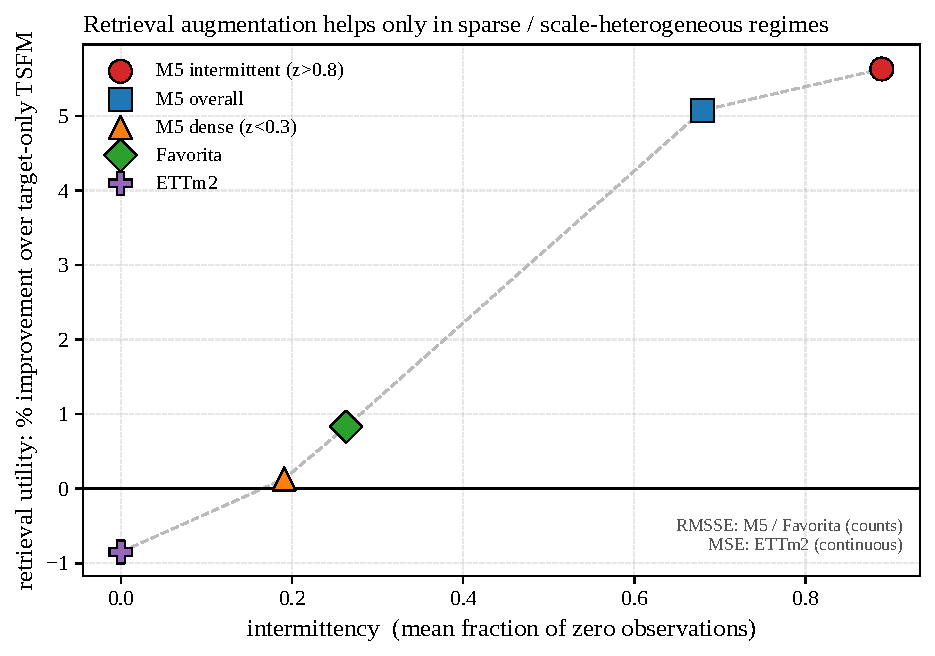
\includegraphics[width=\columnwidth]{../docs/figures/fig4_regimes.pdf}
  \caption{Taxonomy of retrieval regimes. Realised utility of retrieval augmentation over
    the target-only foundation model, plotted against dataset zero-fraction (M5 and
    Favorita in RMSSE, ETTm2 in MSE). Retrieval augmentation pays off in sparse,
    scale-heterogeneous regimes and is neutral-to-harmful on dense continuous channels.}
  \label{fig:regimes}
\end{figure}

\subsection{Held-Out M5 Evaluation: Pre-Registered Criteria and Negative Findings}
\label{sec:m5-caveats}
We report the held-out M5 outcome in full, including the results that do not favour our method. The +5.49\% RMSSE gain over the frozen Chronos-2 backbone is real and its confidence interval excludes zero, but it does \emph{not} generalise into a claim of state-of-the-art forecasting accuracy, for four reasons.

First, the margin over the strongest simple baseline is small. Against LightGBM \cite{lightgbm}, ScaleRAG improves RMSSE by only +0.69\% (95\% CI [+0.57\%, +0.82\%]). Our pre-registered success criterion required at least a 3\% relative improvement over the strongest matched baseline, so this criterion \textbf{fails} despite the interval excluding zero. Statistical significance here is not practical significance: with 30,490 series, a sub-1\% effect is comfortably detectable while remaining operationally negligible.

Second, ScaleRAG \emph{loses the official M5 metric}. On WRMSSE---the dollar-weighted, hierarchical metric that defines the M5 competition---LightGBM (0.8663) and even Seasonal-Naive (0.8697) beat ScaleRAG (1.2231). Our method is mid-pack on the benchmark's own headline metric.

Third, the RMSSE gain does not carry over to absolute-error or probabilistic accuracy. The frozen target-only Chronos-2 backbone is the best model on MASE (0.893 vs.\ our 1.020), WAPE (0.665 vs.\ 0.698), MAE (0.960 vs.\ 1.008), pinball loss (0.289 vs.\ 0.298), and calibration: at a nominal 80\% level, Chronos-2 attains 0.786 empirical coverage while our gated fusion under-covers at 0.698. Retrieval fusion therefore trades typical-case and distributional accuracy for reduced large squared errors on intermittent series.

Fourth, taken together, \textbf{0 of 3 pre-registered success criteria were met} on the held-out panel. We report this rather than re-tuning, because the test split was consumed exactly once by design and any post-hoc adjustment would invalidate it.

The honest reading is that no single method dominates: the winner reorders with the metric. This metric-dependent reordering, rather than a leaderboard position, is the empirical contribution---together with the mechanism-level result of Sec.~\ref{sec:ablation}, which is unambiguous and holds in both regimes.

\subsection{Compute and Efficiency Trade-offs}
\label{sec:compute}
TS-RAG achieves superior accuracy on continuous data but introduces 4.78M trainable parameters and significant VRAM overhead. ScaleRAG's retrieval and restoration stages introduce \emph{zero} trainable parameters; on M5 the only trained component is the LightGBM gate of Sec.~\ref{sec:fusion}, which is orders of magnitude smaller than a neural mixer and requires no pretraining corpus.

Search is \emph{exact} in every configuration reported here---we never approximate the nearest-neighbour set, so accuracy differences cannot be attributed to index quantisation. Two exact implementations are used, matched to scale. The ETTm2 study uses FAISS with a flat CPU-resident \texttt{IndexFlatL2}, which is why Table~\ref{tab:compute} attributes 0\,MB VRAM and 0.607\,ms per window to the retrieval step. Scaling to the full 30,490-series M5 panel makes the CPU path intractable ($\mathcal{O}(n_{\text{query}} \times n_{\text{candidate}})$ at roughly five hours per origin), so for that panel we use a batched GPU implementation of the \emph{same} exact search: the GPU performs a coarse float32 $L_2$ over-fetch, and the final top-$k$ selection, tie-break, and float64 restoration are resolved exactly as in the CPU path. This GPU path was verified bit-for-bit identical to the frozen CPU retriever before any held-out run (maximum absolute difference 0.0); it is an arithmetic acceleration, not a method change.

Table~\ref{tab:compute} gives the full accounting and Fig.~\ref{fig:pareto} plots the resulting accuracy--latency trade-off: on ETTm2, ScaleRAG is Pareto-dominated, being both slower end-to-end (1.038\,ms vs.\ 0.450\,ms per window) and less accurate than the official neural adapter. Fig.~\ref{fig:sensitivity} shows that this conclusion is not an artefact of the neighbour budget---restored-retrieval and fused MSE are stable across $k \in \{5, 10, 20\}$.

% Table 3: Measured compute / storage / parameter accounting, one machine (RTX 5070 Ti,
% sm_120), batch 256, warm-up excluded from all timings.
% Source: reports/phase11a/compute_backbone.json (backbone params/VRAM/latency),
%         reports/phase11a/compute_scalerag.json (ScaleRAG retrieval index/latency/RAM),
%         reports/phase11a/repro_{chronos_bolt_target,tsrag_official}_ettm2.json
%         (full-test wall-clock eval_seconds, used to derive the TS-RAG per-window latency
%         by scaling the measured backbone latency by the wall-clock ratio -- the ARM
%         adds ~4.3% wall time over the frozen backbone).
% ScaleRAG's "storage" is its train-only in-RAM float64 index (contexts + continuations);
% the official TS-RAG knowledge-base pickle (1,528.6 MB, full-series, not train-only) is
% listed alongside it as an unlike-for-unlike storage reference, not a fair comparison
% (ScaleRAG deliberately restricts to a stricter, train-only candidate pool).
% Requires \usepackage{graphicx} for \resizebox (wide 6-column table).
% Layout: two-column journal style (svjour3 twocolumn) -- spans both columns via table*.
% Inside table*, \textwidth is the full two-column text width, so \resizebox{\textwidth}
% constrains the tabular to the spread exactly (in a single-column table it would have
% overflowed the column by ~half the page).
\begin{table*}[t]
  \centering
  \caption{Measured compute, storage, and trainable-parameter accounting (ETTm2, one machine,
    batch 256, warm-up excluded). ScaleRAG's retrieval index is CPU-resident (0 VRAM);
    latency is reported separately for the frozen backbone forward pass and the retrieval
    step, since ScaleRAG's fused forecast requires both.}
  \label{tab:compute}
  \resizebox{\textwidth}{!}{%
  \begin{tabular}{@{}lccccc@{}}
    \toprule
    Component & Train.\ params & Latency / window & Peak VRAM & Peak RAM & Storage \\
    \midrule
    Chronos-Bolt backbone (frozen) & 0 (205.3M) & 0.431\,ms & 1{,}562\,MB & --- & --- \\
    TS-RAG ARM (official)          & 4.78M      & 0.450\,ms ($+4.3\%$) & $\sim$1.6\,GB & --- & 1{,}528.6\,MB$^{\ast}$ \\
    ScaleRAG retrieval (non-neural) & 0          & 0.607\,ms (CPU) & 0 (CPU) & 1{,}245.0\,MB & 1{,}096.2\,MB \\
    \midrule
    ScaleRAG total (backbone + retrieval) & 0 & 1.038\,ms & 1{,}562\,MB & 1{,}245.0\,MB & --- \\
    \bottomrule
  \end{tabular}%
  }
  \\[4pt]
  {\footnotesize $^{\ast}$Full-series official knowledge base (not train-only); listed for
   storage reference, not a like-for-like index-size comparison.}
\end{table*}


\begin{figure}[t]
  \centering
  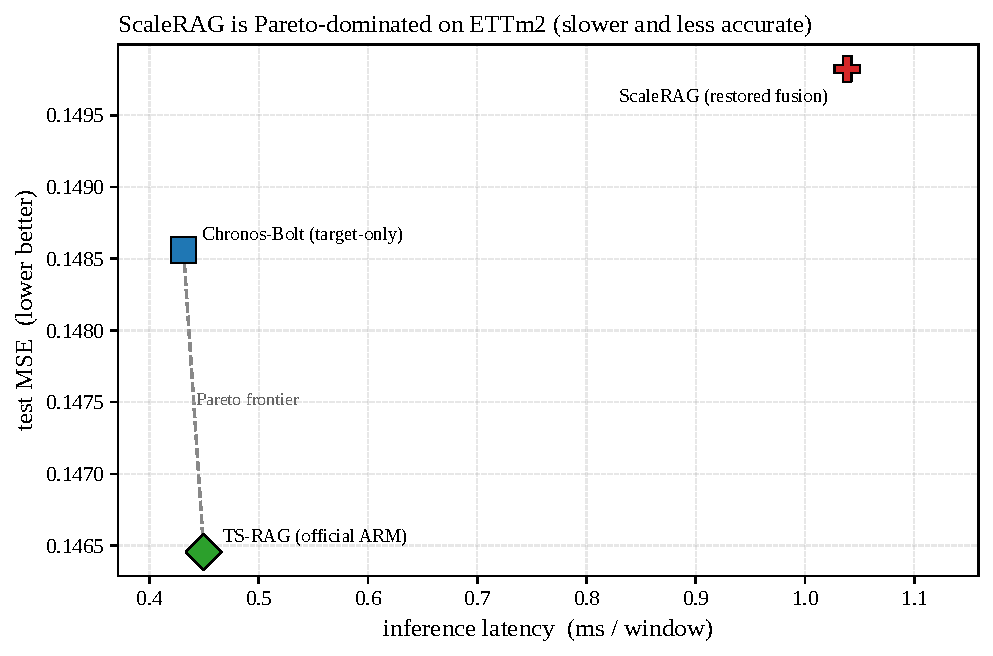
\includegraphics[width=\columnwidth]{../docs/figures/fig5_pareto.pdf}
  \caption{Accuracy versus latency per window on ETTm2. ScaleRAG is Pareto-dominated in
    this regime: the official TS-RAG adapter is both faster end-to-end and more accurate.
    The efficiency argument for ScaleRAG rests on trainable-parameter count and
    deployability, not on wall-clock latency.}
  \label{fig:pareto}
\end{figure}

\begin{figure}[t]
  \centering
  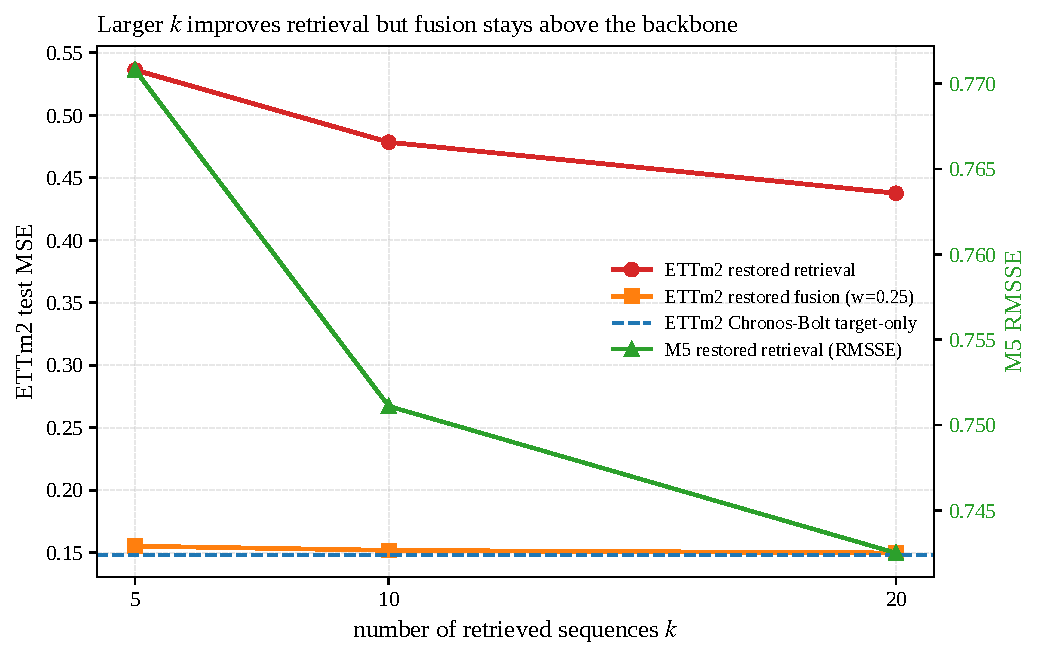
\includegraphics[width=\columnwidth]{../docs/figures/fig6_sensitivity.pdf}
  \caption{Sensitivity to the neighbour budget $k \in \{5, 10, 20\}$ on ETTm2 (mean
    scaling, fusion weight $0.25$). Both restored-retrieval and fused MSE are flat in $k$,
    so the reported outcome is not an artefact of the frozen $k=20$ choice.}
  \label{fig:sensitivity}
\end{figure}

Therefore, explicit statistical restoration is not proposed as a substitute for neural RAG on dense benchmarks, but rather as an operational option for sparse datasets and resource-constrained environments where neural adapters risk scale hallucination, cannot be pretrained, or are impossible to deploy.

\section{Conclusion}
\label{sec:conclusion}

In this paper, we identified and resolved the catastrophic scale mismatch inherent in non-neural retrieval for Time Series Foundation Models. By introducing a mathematical formulation that adds no trainable parameters to the retrieval path---normalizing context prior to indexing and explicitly restoring continuation magnitude post-retrieval using only the query's own statistics---we demonstrated an 85.4\% recovery in retrieval MSE and prevented a 3.8$\times$ forecasting degradation on sparse data. Search remains exact throughout, executed by a flat CPU-resident FAISS index at benchmark scale and by a bit-identical batched GPU implementation of the same exact search on the full 30,490-series M5 panel.

We are deliberate about the parameter accounting. Indexing, search, and scale restoration are entirely parameter-free, and the dense-regime configuration keeps the full pipeline so. The sparse-regime configuration adds exactly one lightweight learned component---a LightGBM gate over six origin-available diagnostic features, fitted on training origins only---which remains three orders of magnitude smaller than the neural mixers it replaces, but which we decline to describe as parameter-free.

Crucially, our empirical analysis establishes a clear \textit{Taxonomy of Retrieval Regimes}. State-of-the-art neural retrieval adapters excel on dense, continuous datasets, where their parameter overhead and retraining requirements buy real accuracy; on ETTm2 our statistical fusion is both slower and less accurate than the official neural adapter, and marginally worse than the frozen backbone it augments. For highly sparse, zero-inflated domains, or where resources preclude training a neural adapter at all, explicit mathematical scale restoration provides a robust, deployable augmentation strategy.

We also report the limits of that claim without qualification. On the held-out M5 panel, ScaleRAG improved squared-error accuracy over its frozen backbone by +5.49\% RMSSE, yet beat the strongest classical baseline by only +0.69\%---below our pre-registered 3\% threshold---lost the official WRMSSE metric to both LightGBM and Seasonal-Naive, and was surpassed by the target-only backbone on MAE, WAPE, MASE, pinball loss, and interval coverage. All three pre-registered success criteria failed. The contribution of this work is therefore a validated mechanism and a regime taxonomy: scale restoration is demonstrably necessary for statistical retrieval to function at all, while the end-to-end value of that retrieval is bounded by regime and by metric. We regard the delineation of that boundary as more useful to practitioners than a leaderboard result, and we leave calibration-preserving fusion---the clearest deficiency our evaluation exposed---to future work.


\bibliographystyle{spmpsci}
\bibliography{references}

\end{document}
